\documentclass[11pt, twocolumn]{article}

\usepackage{graphicx}
\usepackage{url}

\begin{document}

\title{Using machine learning for content-based music analysis}
\author{Matt Hems, Kevin Lopez\\
  Department of Computer Science\\
  Binghamton University\\
\{mhems1, klopez9\}@binghamton.edu}
\maketitle

\begin{abstract}
Over the course of the semester, we worked towards the goal of employing machine
learning to see if content-based music analysis was feasible. Our work consists
of gathering and assembling data annotated with music content and genre labels,
and then training two learners on that dataset. We implement a decision tree
with pre and post pruning capabilities to classify a song’s genre given
information about its content. A k-means clustering learner is also implemented
to classify songs into clusters of similarity and see if this mimics the
song’s genres. Our modest results indicate a need for more (training) data as
well as more variance within the data set.
\end{abstract}

\section{Introduction}
    Before we can analyze machine learning’s application to content-based
analysis, we digress to summarize the musical properties employed by our
algorithm. The features of our data are metrics of a song’s sections, bars,
beats, tatums, tempo, and duration. A section is defined as a part of a song
that encapsulates a single theme (e.g. the intro, the bridge, verses, etc.). A
bar, or measure, is a unit of music that combine to make up a musical idea, or
phrase; phrases, in turn, combine to form sections. A beat is a subdivision of
a bar, usually denoted by percussive instruments in many musical genres. A
tatum is a further subdivision, described by Blimes \cite{blimes} as “an
unconscious and intuitive high-frequency pulse” that allows one to perceive
and predict musical events such as notes and beats. Tempo is the speed of the
song, expressed in beats per minute (bpm). Duration is the length of the song.
    The data set we use is the SALAMI Annotation data \cite{mcgill}, a
compilation of 800 songs annotated with metrics regarding the aforementioned
features as well as its genre. The annotations come from the EchoNest music
platform which itself uses machine learning to annotate songs. For the purposes
of this assignment, we assume all songs are annotated correctly and take these
values at 100\% confidence.

\begin{figure}
  \centering
  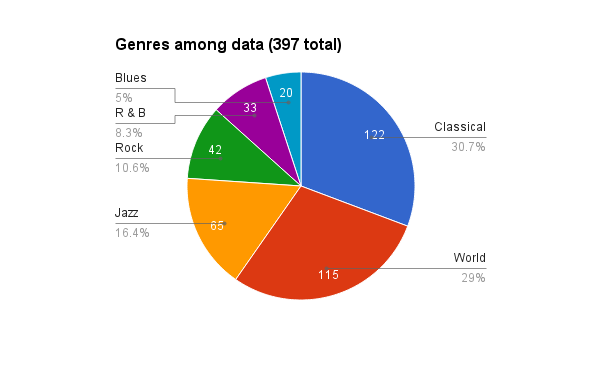
\includegraphics[width=\linewidth]{resources/chart.png}
  \caption{Genre composition of SALAMI database subset}
  \label{fig:chart}
\end{figure}

    Of the 800 songs supplied the SALAMI database, 500 of them came with a
genre  annotation and 400 of those belonged to a genre of non-trivial
frequency. The genres these projects attempt to classify are Blues, R \& B,
Jazz, Rock, Classical, and World. A crucial decision of this project was to
exclude those genres that appeared rarely and also merge those annotations that
belonged to a more general category. For example, the Country genre only
appears eight times in the data set so to classify it would require a level of
precision beyond the scope of this project. Subgenres of classical music, such
as baroque and romantic, were merged into the overarching classical genre,
likewise for rock and alternative rock. See Figure~\ref{fig:chart} for a
complete breakdown of the genres.

\section{Background}
    Music analysis is a topic many machine learning researchers are interested
in. With ties to speech recognition, segmentation, and audio processing,
musical learners are of note for many people across the sciences and arts.
Musical machine learning also has the keen eye of industry, with many startups
and companies racing to be the next craze for music producers and consumers
alike. Websites such as Pandora and mobile applications like Shazam are seeing
commercial success in their ability to recommend and classify music. In this
project, we strive to implement our own learners to experience the challenges
of musical machine learning. We are primarily interested in the topic of genre
classification, that is, given a song and some set of pertaining features, can
the song’s genre be determined. The term genre is used loosely where we make
the simplifying assumption that a song is a member of exactly one genre and
genres form mutually disjoint subsets of the set of all music.

\section{Related Works}
    For the purposes of this assignment and our learning goals, we take
interest in the work of the Laboratory for the Recognition and Organization of
Speech and Audio (LabROSA) of Columbia University \cite{labrosa}. Among other
areas of musical machine learning, they actively research music classification
and similarity estimation. \cite{similarity} presents an optimization of
content-based similarity search by employing the KD tree data structure over a
nearest neighbors approach. The authors list the advantages of such an approach
as ease of implementation and minimal parameter tuning. To combat potential
degradation in higher dimensions, they propose that the tree nodes split on the
axis that most spreads the remaining data. This diverges from our
implementation of a decision tree where the axis with maximum information gain
is selected to split on.
    We see research into music clustering by LabROSA in \cite{olda}. In their
paper, they detail a supervised learning algorithm for temporal-based
clustering of songs. They partition a song into discrete homogenous segments,
e.g. verse, chorus, bridge via Ordinal Linear Discriminant Analysis (OLDA).
This is a learning technique for feature transformation tuned specifically for
music segmentation. This segmentation algorithm provides a partition of a song
into its components - a similar output to what our learners take as input
(sections). Their work develops a latent structural repetition feature that
encapsulates the repetitive patterns of a song \cite{olda}. This feature is
likely influential in a song’s genre classification/clustering. Songs of
different genres tend to subscribe to similar patterns of sections. For
instance, Rock songs may be of the form verse, chorus, verse, chorus, bridge,
verse while the more improvisational genre of Jazz may include instrumentals
and unconventional progressions.
    We again see work in music similarity in \cite{structure}, which discusses
a method for analyzing repeated patterns in music using spectral graph theory.
Vertices represent temporal samples and edges mark equivalent position in a
repetition. The structure is represented internally as a Laplacian matrix so
spectral clustering can be achieved via a k-means approach. Since an interest
of ours is to see if songs can be clustered to resemble their membership in
genres, we are interested in \cite{structure}’s efforts to produce
clusterings. In one of their experiments, the authors analyze sections of a
song to estimate boundaries of sections, e.g. verse, chorus, bridge, etc. We
take note of this achievement because the data used for our project includes
this annotation of both section boundaries and classification.

\section{Results}
\subsection{Decision Tree}
    Our decision tree seeks to classify a song into its genre, given a list of
representative features. These features are tempo, duration, and for the
quantities of bars, beats, tatums, and sections, we have annotations of
quantity and average length. We seek to classify the songs into the genres
Blues, R \& B, Jazz, Rock, World, and Classical. We evaluate our decision tree
using tenfold cross-validation with each song selected randomly. With our
initial implementation, we earn a meager average accuracy rate of 28.7\%, where
the average tree has height 15.4 and 289 vertices.

\begin{figure}
  \centering
  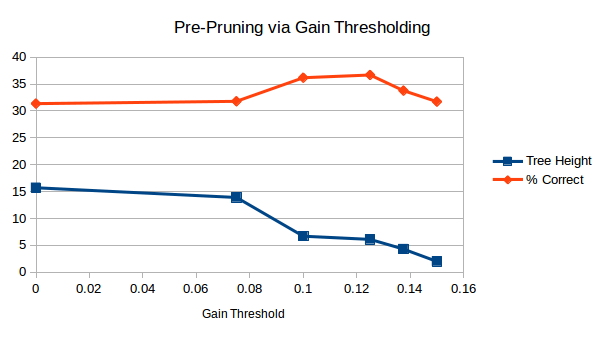
\includegraphics[width=\linewidth]{resources/gain.png}
  \caption{Using cross-validation to find minimum information gain threshold}
  \label{fig:graph}
\end{figure}

\begin{table*}
  \begin{center}
    \begin{tabular}{ |c|c|c|c|c| }
      \hline
      Algorithm & Partition & Height & Number of Vertices & \% Correct \\
      \hline
      No pruning & 8:1 & 15.1 & 289 & 33.48 \\
      No pruning & 9:1 & 15.4 & 289 & 28.68 \\
      Pre-pruning & 8:1 & 5.4 & 21.4 & 35.09 \\
      Pre-pruning & 9:1 & 4.6 & 14.2 & 35.31 \\
      Post-pruning & 8:1:1 & 12.6 & 157.6 & 35.27 \\
      \hline
    \end{tabular}
  \end{center}
  \caption{Decision tree results across pruning methods}
  \label{tab:results}
\end{table*}

    To improve upon this, we first try pre-pruning, where a split’s
information gain must be above a minimum threshold or else the node decomposes
into a leaf whose genre is the most frequent genre in that node’s dataset.
This approach has the advantage of avoiding potentially useless search spaces
at the cost of prematurely abandoning paths that have not had time to mature.
For this approach, we use cross-validation to its intended application: the
selection of a minimum threshold of information gain. We empirically obtain a
minimum threshold of 0.125. Results can be seen in full in Figure~\ref{fig:graph}
where we see the inverse relationship between tree height and accuracy which can
be intuitively understood as complexity (overfitting) versus generalization.
Using this minimum threshold, we achieve an accuracy of 35\%, a boost of 20\%.
It is interesting to note that the average tree now has height 4.6 and 14
vertices. One problem with pre-pruning is its haste to prune an underrealized
path.

    To combat this, we turn to post-pruning, where the tree grows to its
natural depth, and is pruned afterwards. The tree is annotated in a bottom-up
fashion with the error achieved and the hypothetical error if that node was
instead a leaf with its genre as the most abundant genre in its dataset. Once
annotation is complete, the node with the greatest reduction in error is pruned
to a leaf, with any subsequent children being severed completely. This process
is repeated until there exists no node with reduction in error. This has the
advantage of knowing that the leaf is pruned is optimal, yet is algorithmically
expensive. Another downside of post-pruning is its requirement for data. We
need a dataset to train the initial tree on, a dataset to annotate the tree’s
hypothetical error with, and a final dataset to evaluate the tree on. We choose
a 8:1:1 cross-validation scheme to obtain an accuracy rate of 35\% with the
trees being of average height of 12.6 on 157.6 vertices. We note the empirical
support of the theory - that pre-pruning produce the smallest trees and
post-pruning forming a compromise between the two poles with optimal accuracy.
A summary of results can be seen in Table~\ref{tab:results}.

\subsection{k-means Clustering}
    For the k-means clustering algorithm, we wanted to see if genres naturally
clustered together based on the musical qualities exhibited by samples of those
genres, and if so, with which features. For this algorithm, we restricted the
dataset to three different genres (Classical, World, and Jazz) and set k to
three. We designed the k-means clustering algorithm so that we are able to
visualize the learner in two dimensions; the algorithm plots the points in
Euclidean space with each axis representing a different feature.
    First, two features are chosen. The dataset is then partitioned into a
training set (1/3 of the total, or 100 samples, randomly selected) and a
testing set (the other 200 samples). The training set develops the clusters,
choosing to label the clusters based on which labelling proves most accurate;
that is, whichever combination provides the most correctly assigned genres for
the samples in the training data.
% This part of the process is illustrated in Figure 4.
% Then, each point in the testing set is assigned to a cluster, and the
accuracy of the assignment is tested. This process is iterated multiple times,
and the average accuracy is taken. The algorithm is repeated over different
pairs of features.

\begin{table}
  \begin{center}
    \begin{tabular}{ |c|c|c| }
      \hline
      Feature 1 & Feature 2 & \% Correct \\
      \hline
      tempo & num. tatums & 8 \\
      tempo & mean beat length & 12 \\
      num beats & mean beat length & 8 \\
      duration & num. sections & 13 \\
      \hline
    \end{tabular}
  \end{center}
  \caption{Accuracy ratings across various feature pairings}
  \label{tab:accuracy}
\end{table}

    Unfortunately, results were very low for this method. For example, running
the algorithm over the features tempo (in bpm) and average beat length (that
is, the average time interval between beats in the song) resulted in a 13\%
accuracy rating. Other examples can be seen in Table~\ref{tab:accuracy}. This
low prediction rating could be ascribed to the noise factor, since many samples
had low feature confidence ratings, as mentioned in the introduction. It could
also be attributed to the unreliability of the algorithm itself, since k-means
is meant to detect well-defined clusters
% --as seen in Figure 4,
the genres show much overlap. Finally, it may be that the tested genres actually
sound and behave similar to each other, and are thus hard to predict with
respect to the features provided by our dataset. Perhaps with more features to
test on, more obvious groupings could have revealed themselves.
\vfill
\eject

\begin{thebibliography}{9}
\bibitem{blimes}
 J. Blimes, “Timing is of the Essence: Perceptual and Computational
Techniques for
      Representing, Learning, and Reproducing Expressive Timing in Percussive
Rhythm”
\bibitem{mcgill}
      \path{https://ddmal.music.mcgill.ca/ research/salami/annotations}
\bibitem{labrosa}
      \path{http://labrosa.ee.columbia.edu/}
\bibitem{similarity}
      B. McFee, G. Lanckriet. “Large-Scale Music Similarity Search with
Spatial Trees”
\bibitem{olda}
      B. McFee, D. Ellis. “Learning to segment songs with ordinal linear
discriminant analysis”
\bibitem{berenzweig}
      A. Berenzweig, B. Logan, et al. “A Large-Scale Evaluation of Acoustic
and Subjective Music Similarity Measures”.
\bibitem{embeddings}
      B. McFee, G. Lanckriet. “Heterogeneous Embeddings for Subjective Artist
Similarity”
\bibitem{vaizman}
      Y. Vaizman, B. McFee, et al. “Codebook based Audio Feature
Representation for Music Information Retrieval”
\bibitem{structure}
      B. McFee, D. Ellis. “Analyzing song structure with spectral
clustering”
\end{thebibliography}

\end{document}
